\documentclass{standalone}
\usepackage{tikz}
\usepackage{float}
\usepackage{amsmath}
\usepackage{lmodern}
\usepackage{amssymb}
\usetikzlibrary{calc}
\usetikzlibrary{hobby}
\usepackage{nicefrac}
\usetikzlibrary{decorations.markings}
\usetikzlibrary{patterns, patterns.meta}
\usetikzlibrary{shapes}
\usepackage{pgfplots}

\begin{document}


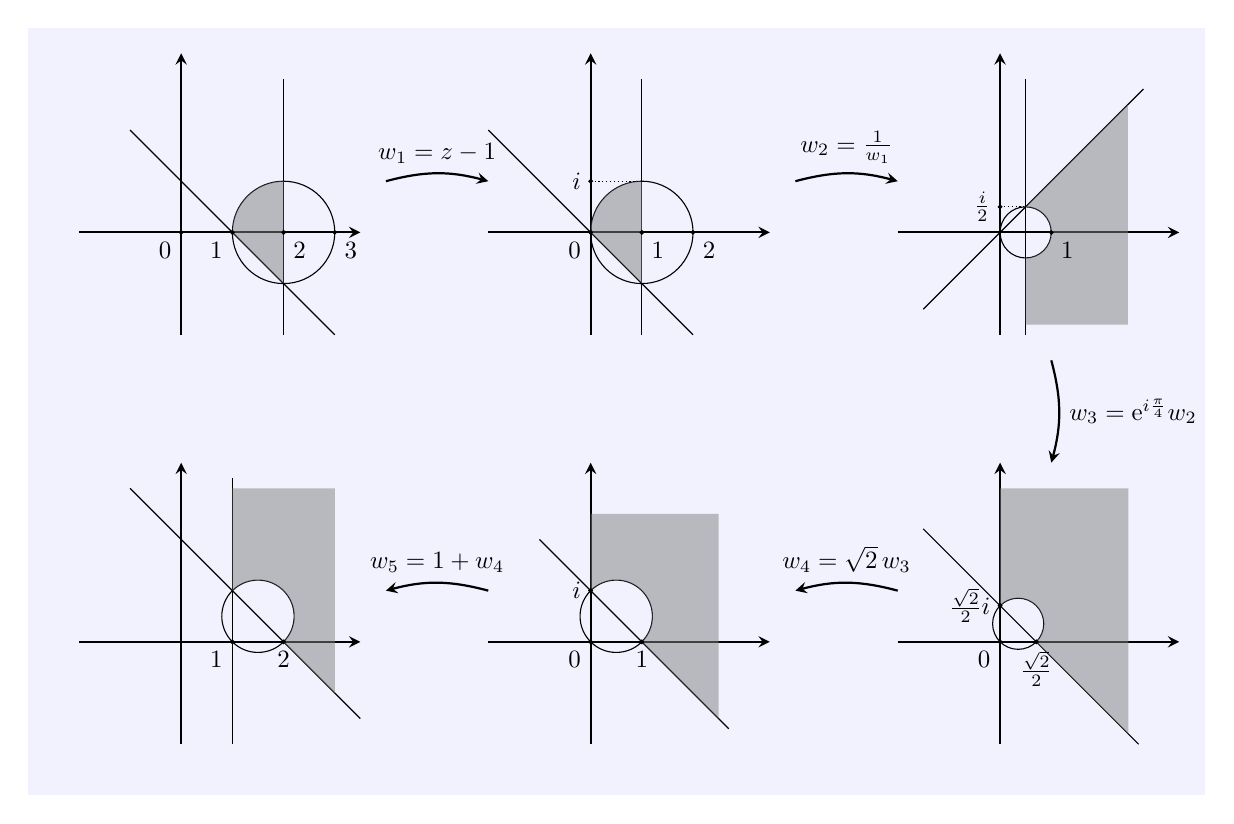
\begin{tikzpicture}[scale=0.65]
    \tikzset{arrowstyle/.style={->, >=stealth}}

    \colorlet{BlueBackground}{blue!5}
    % Background for entire canvas
    \fill[blue!5] (-11,-3) rectangle (12,12);

    % === Figure positions ===
    % We'll define each figure in its own scope with a shift

    \newcommand{\SetupSubfigure}[0]{
    % Function that draws the axes of a subfigure and sets up origin
    \coordinate (O) at (0,0);
    \draw[thick, arrowstyle] ($(O) + (-2,0)$) -- ($(O) + (3.5,0)$);
    \draw[thick, arrowstyle] ($(O) + (0,-2)$) -- ($(O) + (0,3.5)$); 
    }

    % ----------------------
    % First Figure
    \begin{scope}[shift={(-8,8)}]
        \SetupSubfigure
        \draw (2,0) circle(1);
        \draw (-1,2) -- (3,-2);
        \draw (2,-2) -- (2,3);
        \begin{scope}
            \clip (2,-1) -- (1,0) -- (1,1) -- (2,1) -- cycle;
            \fill[gray, opacity=0.5] (2,0) circle(1);
        \end{scope}
        \filldraw (0,0) circle(1pt) node[below left] {\scalebox{0.9}{0}};
        \filldraw (1,0) circle(1pt) node[below left] {\scalebox{0.9}{1}};
        \filldraw (2,0) circle(1pt) node[below right] {\scalebox{0.9}{2}};
        \filldraw (3,0) circle(1pt) node[below right] {\scalebox{0.9}{3}};
    \end{scope}

    % ----------------------
    % Second Figure
    \begin{scope}[shift={(0,8)}]
        \SetupSubfigure
        \draw (1,0) circle(1);
        \draw (-2,2) -- (2,-2);
        \draw (1,-2) -- (1,3);
        \begin{scope}
            \clip (1,-1) -- (0,0) -- (0,1) -- (1,1) -- cycle;
            \fill[gray, opacity=0.5] (1,0) circle(1);
        \end{scope}
        \filldraw (0,0) circle(1pt) node[below left] {\scalebox{0.9}{0}};
        \filldraw (1,0) circle(1pt) node[below right] {\scalebox{0.9}{1}};
        \filldraw (2,0) circle(1pt) node[below right] {\scalebox{0.9}{2}};
        \filldraw (0,1) circle(1pt) node[left] {\scalebox{0.9}{$i$}};
        \draw[densely dotted] (0,1) -- (1,1);
    \end{scope}

    % Arrow from 1st to 2nd
    \draw[arrowstyle, thick, bend left=15] (-4,9) to node[midway, above] {\scalebox{0.9}{$w_1 = z-1$}} (-2,9);

    % ----------------------
    % Third Figure (Middle-right)
    \begin{scope}[shift={(8,8)}]
        \SetupSubfigure
        \draw (1/2,0) circle(1/2);
        \draw (-1.5,-1.5) -- (2.8,2.8);
        \draw (1/2,-2) -- (1/2,3);
        \begin{scope}
            \clip (1/2, -1.8) -- (1/2,-1/2)arc[start angle=-90, end angle=90, radius=1/2] -- (1/2,1/2) -- (2.5,2.5)-- (2.5,-1.8) -- cycle;
            \fill[gray, opacity=0.5] (1/2,-2) -- (1/2,1/2) -- (2.5,2.5) -- (2.5,-2) -- cycle;
        \end{scope}
        \filldraw (1,0) circle(1pt) node[below right] {\scalebox{0.9}{1}};
        \filldraw (0,1/2) circle(1pt) node[left] {\scalebox{0.9}{$\tfrac{i}{2}$}};
        \draw[densely dotted] (0,1/2) -- (1/2,1/2);
    \end{scope}

    % Arrow from 2nd to 3rd
    \draw[arrowstyle, thick, bend left=15] (4,9) to node[midway, above] {\scalebox{0.9}{$w_2 = \frac{1}{w_1}$}} (6,9);

    % ----------------------
    % Fourth Figure 
    \begin{scope}[shift={(8,0)}]
        \SetupSubfigure
        \draw ({sqrt(2)/4},{sqrt(2)/4}) circle(1/2);
        \draw (-1.5,{sqrt(2)/2+1.5}) -- ({sqrt(2)/2 +2},-2);
        \begin{scope}
            \clip ({sqrt(2)/2 +1.8},-1.8) -- ({sqrt(2)/2},0)arc[start angle=-45, end angle=135, radius=1/2] -- (0,3) -- ({sqrt(2)/2 +1.8},3)-- cycle;
            \fill[gray, opacity=0.5] (-3,-3) -- (3,-3) -- (3,3) -- (-3,3) -- cycle;
        \end{scope}
\filldraw (0,0) circle(1pt) node[below left] {\scalebox{0.9}{0}};
\filldraw ({sqrt(2)/2},0) circle(1pt) node[below] {\scalebox{0.9}{$\tfrac{\sqrt{2}}{2}$}};
\filldraw (0,{sqrt(2)/2}) circle(1pt) node[left] {\scalebox{0.9}{$\tfrac{\sqrt{2}}{2}i$}};

    \end{scope}

    % Arrow from 3rd to 4th
    \draw[arrowstyle, thick, bend left=15] (9,5.5) to node[midway, right] {\scalebox{0.9}{$w_3 = \mathrm{e}^{i\frac{\pi}{4}} w_2$}} (9,3.5);

    % ----------------------
    % Fifth Figure (Bottom-left)
    \begin{scope}[shift={(0,0)}]
        \SetupSubfigure
        \draw (1/2,1/2) circle({sqrt(2)/2});
        \draw (-1,2) -- (2.7,-1.7);
        \begin{scope}
            \clip (2.5,-1.5) -- (1,0) 
                  arc[start angle=-45, end angle=135, radius={sqrt(2)/2}] 
                  -- (0,2.5) -- (2.5,2.5) -- cycle;
            \fill[gray, opacity=0.5] (-3,-3) -- (3,-3) -- (3,3) -- (-3,3) -- cycle;
        \end{scope}
        \filldraw (0,0) circle(1pt) node[below left] {\scalebox{0.9}{0}};
        \filldraw (1,0) circle(1pt) node[below] {\scalebox{0.9}{1}};
        \filldraw (0,1) circle(1pt) node[left] {\scalebox{0.9}{$i$}};

    \end{scope}

    % Arrow from 4th to 5th
    \draw[arrowstyle, thick, bend right=15] (6,1) to node[midway, above] {\scalebox{0.9}{$w_4 = \sqrt{2}\,w_3$}} (4,1);

    % ----------------------
    % Sixth Figure (Bottom-right)
    \begin{scope}[shift={(-8,0)}]
        \coordinate (O) at (0,0);
        \draw[thick, arrowstyle] ($(O) + (-2,0)$) -- ($(O) + (3.5,0)$);
        \draw[thick, arrowstyle] ($(O) + (0,-2)$) -- ($(O) + (0,3.5)$);
        \draw (3/2,1/2) circle({sqrt(2)/2});
        \draw (-1,3) -- (3.5,-1.5);
        \draw (1,-2) -- (1,3.2);
        \begin{scope}
            \clip (3,-1) -- (2,0) 
                  arc[start angle=-45, end angle=135, radius={sqrt(2)/2}] 
                  -- (1,3) -- (3,3) -- cycle;
            \fill[gray, opacity=0.5] (-3.5,-3.5) -- (3.5,-3.5) -- (3.5,3.5) -- (-3.5,3.5) -- cycle;
        \end{scope}
        \filldraw (1,0) circle(1pt) node[below left] {\scalebox{0.9}{1}};
        \filldraw (2,0) circle(1pt) node[below] {\scalebox{0.9}{2}};

    \end{scope}

    % Arrow from 4th to 5th
    \draw[arrowstyle, thick, bend right=15] (-2,1) to node[midway, above] {\scalebox{0.9}{$w_5 = 1+w_4$}} (-4,1);


\end{tikzpicture}

\end{document}
